\section{Introduction}
\label{sec:intro}

Understanding the internal representations learned by neural networks has
long been a central goal of interpretability research. Early work visualized
or attributed units in image
classifiers~\cite{ZeilerFergus2014,SimonyanEtAl2014,BauEtAl2017,KimEtAl2018}.
More recent work on large language models has used probing
classifiers~\cite{AlainBengio2017,HewittLiang2019,Belinkov2022}, concept
directions~\cite{ZouEtAl2023}, and sparse
decompositions~\cite{CunninghamEtAl2023} to recover human-interpretable
features as linear structure in hidden states. This goal is both scientific
and practical: once a feature can be localized, researchers can audit,
monitor, and intervene on it. Interpretability can therefore help predict and
steer model behaviour in ways that black-box evaluation alone cannot.

Extending this program to vision--language models (VLMs) presents a distinct
challenge. A VLM maps an image to visual tokens that are processed by a
language decoder~\cite{LiuEtAl2023LLaVA,WangEtAl2024Qwen2VL,
BaiEtAl2025Qwen25VL}. These tokens encode the visual content on which the
model reasons. Unlike text tokens, however, they have no discrete identities
drawn from a fixed vocabulary. A visual token can entangle object category,
appearance, scale, position, and scene context, leaving no simple ground truth
for what it should represent. Existing studies have therefore interpreted VLM
internals largely through language: they explain neurons, embedding
components, and sparse features by projecting them onto words or
captions~\cite{OikarinenWeng2023,GandelsmanEtAl2024,BhallaEtAl2024,
NeoEtAl2025,ZaigrajewEtAl2025,PapadimitriouEtAl2025,PachEtAl2025}. Such
vocabulary-level descriptions depend on a potentially noisy naming step and
do not directly characterize visual properties that are difficult to express
as object nouns, such as attributes or the binding of properties to objects.
A systematic account of VLM representations therefore requires evaluation
grounded directly in visual concepts.

We introduce a framework for systematically evaluating VLM representations
across multiple levels of visual abstraction: object category at the token and
image levels, object attributes, and the binding of properties to objects. We
estimate category directions from controlled image contrasts and, at each
label-free level, use a common read-out: a margin pooled over visual tokens
and calibrated against a random-direction floor. This design helps separate
representational signal from artifacts of the read-out and enables consistent
comparisons across models within each concept level.

\begin{figure}
    \centering
    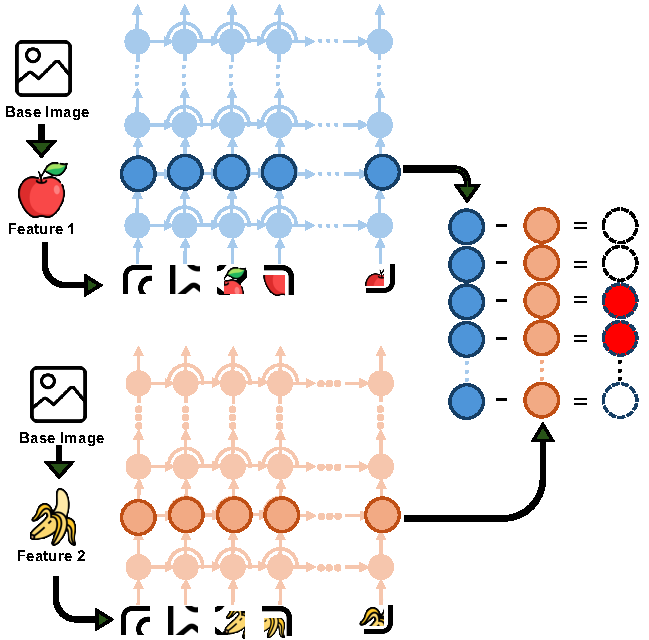
\includegraphics[width=\linewidth]{figs/step1_extraction.pdf}
    \caption{Step 1: contrast representation extraction. We paste two target figure on the same base image. }
    \label{fig:placeholder}
\end{figure}

First, we use controlled visual interventions
to identify what carries a feature. A supervised probe can establish that a
property is decodable, but not that it is encoded by the intended object: in
natural images, a category covaries with scene context, framing, and object
scale, and a probe may exploit any of these
signals~\cite{AlainBengio2017,HewittLiang2019}. We instead construct matched
image pairs that differ only in which object occupies the same location.
Subtracting their representations cancels the shared scene, edit, and
category-independent object effects, isolating a category-relative direction
without a fitted probe. Second, we evaluate representations across levels of
granularity. Strong category encoding does not imply equally strong encoding
of attributes or relations. Moving from token-level category to image-level
presence, attributes, and binding reveals where linear feature structure
remains accessible and where it breaks down.

In summary, our contributions are threefold:
\begin{mitemize}
\item We develop a pipeline for identifying VLM feature directions through
    controlled image interventions. Matched image pairs that differ in one
    object category isolate category-relative directions by cancellation,
    without requiring manual or LLM-generated descriptions of those
    directions.
\item We introduce an evaluation metric for VLM interpretability: the gap
    between a label-free pooled-margin read-out and a calibrated
    random-direction floor. The metric applies to datasets spanning multiple
    levels of visual concepts.
\item We evaluate open-weight VLMs cross different model families and sizes and our methods outperform most of the other interpretablility methods. 
\end{mitemize}
